\documentclass[11pt,a4paper]{article}
\usepackage[T1]{fontenc}\usepackage{lmodern}
\usepackage[margin=22mm]{geometry}
\usepackage{amsmath,amssymb,graphicx,booktabs,array,tabularx,enumitem}
\usepackage{xcolor}
\usepackage[colorlinks=true,linkcolor=blue!45!black,citecolor=blue!45!black,urlcolor=blue!45!black]{hyperref}
\setlength{\parindent}{0pt}\setlength{\parskip}{5pt}\setlength{\emergencystretch}{2em}
\setlist[itemize]{leftmargin=*,itemsep=2pt}
\newcommand{\SCNR}{\operatorname{SCNR}}\newcommand{\SINR}{\operatorname{SINR}}\newcommand{\Ree}{\operatorname{Re}}\newcommand{\diag}{\operatorname{diag}}
\title{Initial Solution Derivation and Simulation Validation\\\large Clutter-Aware Near-Field RIS--ISAC with Learning to Optimize}
\author{Muneef Mohammed\\\small Research prototype for advisor discussion}
\date{November 2026}
\begin{document}\maketitle
\begin{abstract}
This note turns the proposed initial RIS-assisted system into an explicit narrowband, reciprocal point-scatterer model, derives a receive-filter solution and beamforming/phase derivatives, and implements a feasible-update optimization prototype. Learning is introduced through a geometry-conditioned phase initializer and layer-specific optimization steps. The learned parameters are fitted offline using a derivative-free cross-entropy method; this is a learned unrolled optimizer, not a backpropagation-trained deep neural network. The accompanying experiments use synthetic ideal-information channels and report all failed initializations. They validate implementation and establish initial comparisons, not global optimality, robust feasibility, physical hardware performance, or the complete PhD proposal.
\end{abstract}

\section{Scope and explicit assumptions}
The model has $N$ colocated transmit/receive array coordinates, an $M$-element passive RIS, $K$ single-antenna users, one target, and $L$ clutter scatterers. Identical reciprocal array coordinates are a simplifying idealization; residual self-interference is assumed perfectly canceled. The prototype is two-dimensional, narrowband, static, and ideal-information. There is no Doppler, waveform bandwidth optimization, channel estimation, tracking, hardware phase quantization, mutual coupling, polarization model, or calibrated array/RIS radiation pattern. Unit-modulus RIS coefficients and scalar free-space propagation form an illustrative link model, not an electromagnetic validation.

In particular, the uncertainty set in the proposal is specialized to a singleton. No adversarial or stochastic robust constraint has been solved. Training/test geometry variation and a clutter-distribution shift do not change this fact. The target state and clutter covariance ingredients are known to this ideal-information controller; replacing them with estimates is future work.

Learning update parameters is motivated by unfolded beamforming work~\cite{nguyen2023unfolding}. Replacing expensive computations is a separate next step, consistent with the distinction between iteration count and per-iteration cost in~\cite{avrahami2026approx}. This implementation retains exact small linear solves.

\section{Near-field signal model}
Let $\mathbf b_n$, $\mathbf r_m$, and $\mathbf p_j$ be base-station, RIS-element, and terminal/scatterer coordinates. For wavelength $\lambda$, define the scalar propagation coefficient
\begin{equation}
 f(\mathbf a,\mathbf b)=\frac{\lambda}{4\pi\|\mathbf a-\mathbf b\|}
 \exp\!\left(-\mathrm i\frac{2\pi}{\lambda}\|\mathbf a-\mathbf b\|\right).
\end{equation}
It retains element-dependent spherical distances. Set $G_{mn}=f(\mathbf r_m,\mathbf b_n)$, $[\mathbf r_j]_m=f(\mathbf p_j,\mathbf r_m)$ and $[\mathbf d_j]_n=b_0 f(\mathbf p_j,\mathbf b_n)$, where $b_0$ is a specified direct-path amplitude attenuation. Let $\phi_m=e^{\mathrm i\theta_m}$. The forward channel is
\begin{equation}\label{eq:v}
 \mathbf v_j=\mathbf d_j+\mathbf G^T\diag(\boldsymbol\phi)\mathbf r_j.
\end{equation}
The convention is $y_j=\mathbf v_j^T\mathbf x+n_j$, not $\mathbf v_j^H\mathbf x+n_j$. Every transpose and conjugate in the code follows this convention.

For independent unit-variance data symbols $\mathbf s$, transmit
\begin{equation}
 \mathbf x=\mathbf W\mathbf s,\qquad \mathbb E[\mathbf s\mathbf s^H]=\mathbf I,
 \qquad \mathbf Q=\mathbf W\mathbf W^H.
\end{equation}
There is no additional dedicated sensing stream in this initial model. Thus
\begin{equation}\label{eq:sinr}
 \gamma_k(\mathbf W,\boldsymbol\theta)=
 \frac{|\mathbf v_k^T\mathbf w_k|^2}
 {\sum_{i\ne k}|\mathbf v_k^T\mathbf w_i|^2+\sigma_c^2}.
\end{equation}

Index the target by $0$ and clutter by $\ell=1,\ldots,L$. The code stores users first, then target, then clutter. Reciprocity gives the echo model
\begin{equation}
 \mathbf y_r=\alpha_0\mathbf v_0\mathbf v_0^T\mathbf x+
 \sum_{\ell=1}^{L}\alpha_\ell\mathbf v_\ell\mathbf v_\ell^T\mathbf x+\mathbf n_r,
 \qquad\mathbb E[\mathbf n_r\mathbf n_r^H]=\sigma_r^2\mathbf I.
\end{equation}
Assume independent zero-mean scattering coefficients with $\mathbb E|\alpha_j|^2=\beta_j$, independent of symbols and noise. Cross-scatterer terms then disappear in the ensemble covariance. The model permits one RIS interaction on each leg of a target/clutter echo through the product in~\eqref{eq:v}; it excludes other higher-order interactions.

The illustrative scalar radar normalization is $\beta_j=4\pi\sigma_j/\lambda^2$, with $\sigma_j$ an assigned point-scatterer radar cross section. This matches the elementary direct-path scalar radar scaling under the chosen one-way propagation convention; it does not calibrate RIS scattering efficiency.

Define $\mathbf z_j=\mathbf v_j^T\mathbf W$, $q_j=\|\mathbf z_j\|_2^2$, and $r_j=\mathbf u^H\mathbf v_j$. Then
\begin{subequations}\label{eq:cov}
\begin{align}
 \mathbf R_t&=\beta_0q_0\mathbf v_0\mathbf v_0^H,\\
 \mathbf R_c&=\sum_{\ell=1}^{L}\beta_\ell q_\ell\mathbf v_\ell\mathbf v_\ell^H+\sigma_r^2\mathbf I,\\
 S&=\mathbf u^H\mathbf R_t\mathbf u=\beta_0|r_0|^2q_0,\\
 D&=\mathbf u^H\mathbf R_c\mathbf u=\sum_{\ell=1}^{L}\beta_\ell|r_\ell|^2q_\ell+\sigma_r^2\|\mathbf u\|_2^2,\\
 \SCNR&=S/D.
\end{align}
\end{subequations}
The clutter covariance is signal- and RIS-dependent. It is recomputed after every design change.

\section{Optimization and exact receive-filter update}
The implemented nominal design objective is
\begin{equation}\label{eq:problem}
 \max_{\mathbf W,\boldsymbol\theta,\mathbf u}\ \frac{S}{D}
 \quad\text{s.t.}\quad
 \gamma_k\geq\Gamma\ (\forall k),\quad
 \|\mathbf W\|_F^2\leq P,\quad\|\mathbf u\|_2=1,
\end{equation}
with unit-modulus RIS coefficients enforced by $\boldsymbol\phi=e^{\mathrm i\boldsymbol\theta}$. This non-convex problem is not globally solved by the proposed heuristic.

For fixed $\mathbf W,\boldsymbol\theta$, $\mathbf R_c\succ0$. Since $\mathbf R_t$ has rank one, Cauchy--Schwarz in whitened coordinates gives
\begin{align}
 \frac{|\mathbf u^H\mathbf v_0|^2}{\mathbf u^H\mathbf R_c\mathbf u}
 &\leq\mathbf v_0^H\mathbf R_c^{-1}\mathbf v_0,\\
 \mathbf u^\star&=\frac{\mathbf R_c^{-1}\mathbf v_0}{\|\mathbf R_c^{-1}\mathbf v_0\|_2}.
\end{align}
The implementation solves a linear system instead of explicitly forming $\mathbf R_c^{-1}$. This is a global solution only to the receive-filter subproblem. With the exact receiver, the envelope theorem permits gradients of the reduced objective to be computed while holding $\mathbf u=\mathbf u^\star$ fixed, away from degenerate zero-signal cases.

\section{Beamforming and RIS derivatives}
For numerical optimization and derivative testing, define
\begin{equation}\label{eq:loss}
 \mathcal L=-\log(S/D)+\rho\sum_k\delta_k^2,\qquad
 \delta_k=[\log\Gamma-\log\gamma_k]_+.
\end{equation}
The penalty is not a feasibility certificate. In accepted feasible iterates it is zero; feasibility is checked separately.

\subsection{Wirtinger derivative with respect to the beamformers}
Let $\mathbf H_k=\mathbf v_k^*\mathbf v_k^T$ and
\begin{equation}
 \mathbf B_j=\beta_j|\mathbf u^H\mathbf v_j|^2\mathbf v_j^*\mathbf v_j^T.
\end{equation}
Since $\partial\operatorname{tr}(\mathbf W^H\mathbf B\mathbf W)/\partial\mathbf W^*=\mathbf B\mathbf W$ for Hermitian $\mathbf B$,
\begin{equation}\label{eq:gw}
 \frac{\partial\mathcal L}{\partial\mathbf W^*}
 =-\frac{\mathbf B_0\mathbf W}{S}
 +\frac{\sum_{\ell=1}^L\mathbf B_\ell\mathbf W}{D}
 -2\rho\sum_k\delta_k\frac{\partial\log\gamma_k}{\partial\mathbf W^*}.
\end{equation}
Write $s_k=|\mathbf v_k^T\mathbf w_k|^2$ and $I_k=\sum_{i\ne k}|\mathbf v_k^T\mathbf w_i|^2+\sigma_c^2$. Columnwise,
\begin{equation}\label{eq:gsinr}
 \frac{\partial\log\gamma_k}{\partial\mathbf w_i^*}=
 \begin{cases}\mathbf H_k\mathbf w_k/s_k,&i=k,\\-\mathbf H_k\mathbf w_i/I_k,&i\ne k.\end{cases}
\end{equation}
For a real-valued objective, the gradients with respect to Cartesian coordinates are $2\Ree(\partial\mathcal L/\partial\mathbf W^*)$ and $2\operatorname{Im}(\partial\mathcal L/\partial\mathbf W^*)$. The step size in the implementation absorbs this factor of two.

\subsection{RIS-phase derivative}
The phase Jacobian includes both outgoing and returning target/clutter propagation. From~\eqref{eq:v},
\begin{equation}
 \dot{\mathbf v}_{jm}\equiv\frac{\partial\mathbf v_j}{\partial\theta_m}
 =\mathrm i e^{\mathrm i\theta_m}[\mathbf r_j]_m\mathbf G_{m,:}^{T}.
\end{equation}
Define $\dot{\mathbf z}_{jm}=\dot{\mathbf v}_{jm}^{T}\mathbf W$ and $\dot r_{jm}=\mathbf u^H\dot{\mathbf v}_{jm}$. Then
\begin{align}
 \dot q_{jm}&=2\Ree\!\left(\sum_i z_{ji}^*\dot z_{jmi}\right),\\
 \dot p_{jm}&=\beta_j\left[2\Ree(r_j^*\dot r_{jm})q_j+|r_j|^2\dot q_{jm}\right],\\
 \frac{\partial\log(S/D)}{\partial\theta_m}
 &=\frac{\dot p_{0m}}{S}-\frac{\sum_{\ell=1}^L\dot p_{\ell m}}{D}.
\end{align}
Here vector inner products mean summation over the transmitted streams. For communication,
\begin{align}
 \dot s_{km}&=2\Ree\left[(\mathbf v_k^T\mathbf w_k)^*(\dot{\mathbf v}_{km}^T\mathbf w_k)\right],\\
 \dot I_{km}&=\sum_{i\ne k}2\Ree\left[(\mathbf v_k^T\mathbf w_i)^*(\dot{\mathbf v}_{km}^T\mathbf w_i)\right],\\
 \frac{\partial\mathcal L}{\partial\theta_m}
 &=-\frac{\dot p_{0m}}{S}+\frac{\sum_\ell\dot p_{\ell m}}{D}
 -2\rho\sum_k\delta_k\left(\frac{\dot s_{km}}{s_k}-\frac{\dot I_{km}}{I_k}\right).
\end{align}
All expressions are implemented analytically in \texttt{model.py}. Tests recompute the optimal receive filter at perturbed inputs, checking the reduced-objective gradient as well as the complex-conjugation convention.

\section{Exact fixed-direction power repair}
Given candidate beam directions $\mathbf t_i=\mathbf w_i/\|\mathbf w_i\|_2$, write $\mathbf w_i=\sqrt{p_i}\mathbf t_i$. For a fixed RIS, set $a_{ki}=|\mathbf v_k^T\mathbf t_i|^2$. QoS becomes
\begin{equation}
 p_k\geq\sum_{i\ne k}\frac{\Gamma a_{ki}}{a_{kk}}p_i+\frac{\Gamma\sigma_c^2}{a_{kk}}.
\end{equation}
Define $F_{ki}=\Gamma a_{ki}/a_{kk}$ for $i\ne k$, $F_{kk}=0$, and $b_k=\Gamma\sigma_c^2/a_{kk}$. For positive direct gains, nonnegative $\mathbf F$, and $\rho(\mathbf F)<1$,
\begin{equation}
 \mathbf p_{\min}=(\mathbf I-\mathbf F)^{-1}\mathbf b
\end{equation}
is the componentwise minimum feasible power vector. Indeed, the nonnegative inverse is $\sum_{q=0}^{\infty}\mathbf F^q$, and every feasible vector dominates $\mathbf p_{\min}$. Therefore fixed-direction feasibility under the sum-power bound requires $\mathbf 1^T\mathbf p_{\min}\leq P$.

The implemented repair scales $\mathbf p_{\min}$ by $c=P/(\mathbf1^T\mathbf p_{\min})\geq1$. Since
\begin{equation}
 c\mathbf p_{\min}-\mathbf F(c\mathbf p_{\min})=c\mathbf b\geq\mathbf b,
\end{equation}
all nominal QoS inequalities remain satisfied. Common scaling increases sensing SCNR when the spatial design is fixed and receiver noise is positive. This repair is exact for fixed directions only; it is neither the closest Euclidean projection onto the full feasible set nor a certificate of global problem infeasibility when it fails.

The candidate is rejected if its directions fail these conditions. The previous feasible iterate is retained. A final check verifies actual SINRs, power, and RIS modulus. If initial zero-forcing plus power allocation fails, the prototype reports an initialization failure and does not assert that the full joint problem is infeasible.

\section{Conventional and learned algorithms}
\subsection{Feasible-update reference algorithm}
Starting from a physics-based RIS phase choice and zero-forcing beam directions:
\begin{enumerate}
\item Allocate powers using the fixed-direction repair. If this fails, record failure.
\item Solve the receive-filter linear system and evaluate the gradients.
\item Normalize the beamformer gradient by its Frobenius norm and the phase gradient by its root-mean-square magnitude.
\item Form a beamformer step, project onto the power ball, and form a phase step.
\item Repair powers for the new directions and phases; reject infeasible candidates.
\item Optionally backtrack both step sizes by $1/2$, up to seven trials, accepting only non-decreasing SCNR.
\item Return the best feasible visited iterate, with its freshly recomputed receive filter.
\end{enumerate}
The comparison labels use ``PGA'' as shorthand for projected gradient steps plus fixed-direction repair. This is a constrained heuristic; standard convergence claims for Euclidean projected gradient do not automatically apply to the additional repair map. Keeping the best feasible iterate ensures monotone reported incumbent quality, not convergence to a stationary or global optimum.

\subsection{Learning before the solver}
Construct three unit-modulus RIS dictionaries focusing toward the target and each of the two users. For point $j$, use the direct matched beam $\mathbf b_j=\mathbf d_j^*/\|\mathbf d_j\|_2$ and dictionary entry
\begin{equation}
 c_{jm}=\exp\{-\mathrm i\arg([\mathbf r_j]_m[\mathbf G\mathbf b_j]_m)\}.
\end{equation}
For feature vector $\mathbf f=[1,(x_0-1.35)/.35,(y_0-.975)/.225]^T$, learn a $3\times3$ real matrix $\mathbf A$ and weights $\boldsymbol\omega=\operatorname{softmax}(\mathbf A^T\mathbf f)$. Initialize
\begin{equation}
 \theta_m^{(0)}=\arg\left(\sum_{j\in\{0,\mathrm{user1},\mathrm{user2}\}}\omega_j c_{jm}\right).
\end{equation}
This is a small, geometry-conditioned learned initializer with nine parameters, not a GNN or a learned channel estimator. Beam directions remain analytically initialized by zero forcing.

\subsection{Learning inside the solver}
For $T=8$ unfolded layers, learn $\alpha_t$ and $\eta_t$:
\begin{align}
 \widetilde{\mathbf W}^{(t+1)}&=\Pi_{\|\cdot\|_F^2\leq P}
 \left[\mathbf W^{(t)}-\alpha_t\frac{\mathbf g_W^{(t)}}{\max(\|\mathbf g_W^{(t)}\|_F,\epsilon)}\right],\\
 \widetilde{\boldsymbol\theta}^{(t+1)}&=\boldsymbol\theta^{(t)}-
 \eta_t\frac{\mathbf g_\theta^{(t)}}{\max(\sqrt{M^{-1}\|\mathbf g_\theta^{(t)}\|_2^2},\epsilon)}.
\end{align}
Power repair and rejection follow each layer. Sigmoid maps bound $\alpha_t\in(.005,.4)$ and $\eta_t\in(.005,.8)$; these are prototype hyperparameter ranges, not theoretical stability bounds. There are 16 inside-only parameters and 25 combined before/inside parameters.

\subsection{Offline learning and data separation}
The prototype uses the cross-entropy method (CEM): sample 20 parameter vectors per generation, score them on 64 training geometries, retain five elites, and update a Gaussian sampling distribution for 15 generations. Validation selects the checkpoint using 32 separate geometries. Three random training seeds are run. CEM is derivative-free offline meta-optimization; online updates use the derived analytical gradients. This route requires only NumPy and SciPy and does not pretend to implement backpropagation through an unfolding network.

The training score is mean clipped natural-log SCNR for accepted feasible outputs and $-30$ for failed outputs. Thus infeasible instances remain in training and evaluation. A 27-setting fixed-method grid (three initializations and three steps for each variable block) is selected on validation data. The experiments do not equate offline tuning budgets across methods.

\section{Simulation configuration and validation}
The array and geometry parameters are explicitly fixed for a short-range prototype, not a UAV deployment:
\begin{center}\small
\begin{tabular}{ll}\toprule
Parameter & Value\\\midrule
$N,M,K,L$ & $6,12,2,3$\\
Wavelength & $0.1$ m (approximately 3 GHz)\\
BS aperture; RIS aperture & $0.35$ m; $0.55$ m\\
BS coordinates & $x=0$, uniformly spaced $y\in[-.175,.175]$ m\\
RIS coordinates & $x=.65$, uniformly spaced $y\in[.15,.70]$ m\\
Users & $x\sim U[1,1.9]$, $y\sim U[-.8,.15]$ m\\
Target & $x\sim U[1,1.7]$, $y\sim U[.75,1.2]$ m\\
Clutter & Gaussian offsets from target, standard deviation $.22$ m\\
Clutter clipping & $x\geq .85$ m\\
$P,\Gamma,b_0$ & $1$, $2$ (3.01 dB), $.35$\\
$\sigma_c^2,\sigma_r^2$ & $10^{-6},10^{-9}$ in model power units\\
Target RCS; clutter RCS & $.05$ m$^2$; uniform $[.03,.15]$ m$^2$\\
Train / validation / test & $64/32/128$ geometries\\
Shift test & 128 fresh geometries, clutter RCS $\times3$, spread $.12$ m\\
Unfolding depth & 8\\\bottomrule
\end{tabular}
\end{center}
The arrays need not have half-wavelength spacing. Spherical propagation is used directly. The aperture-based Fraunhofer distances are approximately $2.45$ m and $6.05$ m for the BS and RIS, respectively; individual link regimes depend on distance and aperture. These dimensional choices establish a near-field numerical regime, not measured propagation fidelity.

\subsection{Checks actually executed}
Analytical gradients were compared with central finite differences on all real and imaginary beamforming entries and all RIS phases for five random states. The step was $10^{-6}$ and the optimal receiver was recomputed at perturbed points. The maximum relative gradient error was $1.35e-10$. Independent generalized-eigenvalue receiver verification gave maximum relative error $1.17e-15$. A separate 128-instance zero-phase initialization test accepted 103 cases; failures were retained. The accepted power limit and phase modulus were satisfied to floating-point tolerance.

\subsection{Held-out simulation results}
Table~\ref{tab:results} uses 128 held-out geometries. Learned-method entries average the three training seeds; conditional SCNR averages use each model's own feasible subset and must not be interpreted as paired comparisons. ``Feasible'' refers to nominal communication QoS and hardware constraints, not a sensing detection guarantee. No algorithm repairs failed initializations in this prototype.

\begin{table}[!htbp]\centering\small
\begin{tabular}{lrrrr}\toprule
Method & Feasible (\%) & Mean SCNR (dB) & Median (ms) & p95 (ms)\\\midrule
Initialization & 81.25 & -5.21 & 0.31 & 0.53 \\
Fixed steps (8) & 81.25 & 2.36 & 3.74 & 5.89 \\
Learn before & 82.29 & 2.15 & 3.85 & 6.20 \\
Learn inside & 81.25 & 2.84 & 3.76 & 5.99 \\
Before + inside & 81.77 & 2.66 & 3.84 & 6.54 \\
Backtracking (80) & 81.25 & 3.16 & 126.62 & 179.13 \\
\bottomrule\end{tabular}
\caption{Actual synthetic test results and batch-one solver timings. Learned timing entries are means of per-seed medians/p95 values, not pooled quantiles.}\label{tab:results}\end{table}

Runtime is measured with \texttt{perf\_counter} on this shared Linux CPU environment using NumPy complex128 and one OpenBLAS thread. Each method uses three repetitions over 32 batch-one inputs. Timing includes initialization, receiver solves, gradient steps, power repair, candidate evaluation, and final checks. It excludes offline learning and synthetic channel/feature construction. It also excludes sensing acquisition, channel estimation, RIS configuration, and queueing, none of which is simulated. Consequently these numbers are solver timings, not end-to-end deployment latency. Median synthetic input preparation took 0.119 ms; this is not an estimator timing. Offline training of all nine learned models took 61.21 s.

On geometries feasible for both the learned and fixed-step methods, the seed-averaged paired SCNR gain was 0.479 dB for inside-only learning, 0.322 dB for combined before/inside learning, and -0.104 dB for before-only learning. The corresponding geometry-bootstrap 95\% intervals were [0.370, 0.600], [0.213, 0.436], and [-0.221, 0.006] dB. These intervals hold the three trained models fixed and do not capture all training-distribution or model uncertainty.

The combined architecture did not consistently exceed inside-only learning. Before-only learning traded a small feasibility change for lower paired sensing quality. There is no demonstrated runtime reduction relative to the equally shallow eight-step baseline; the 80-step reference spends more time and attains higher average sensing quality. The results support a modest learned-step benefit in this pilot, not a general L2O superiority claim.

\begin{figure}[!htbp]\centering
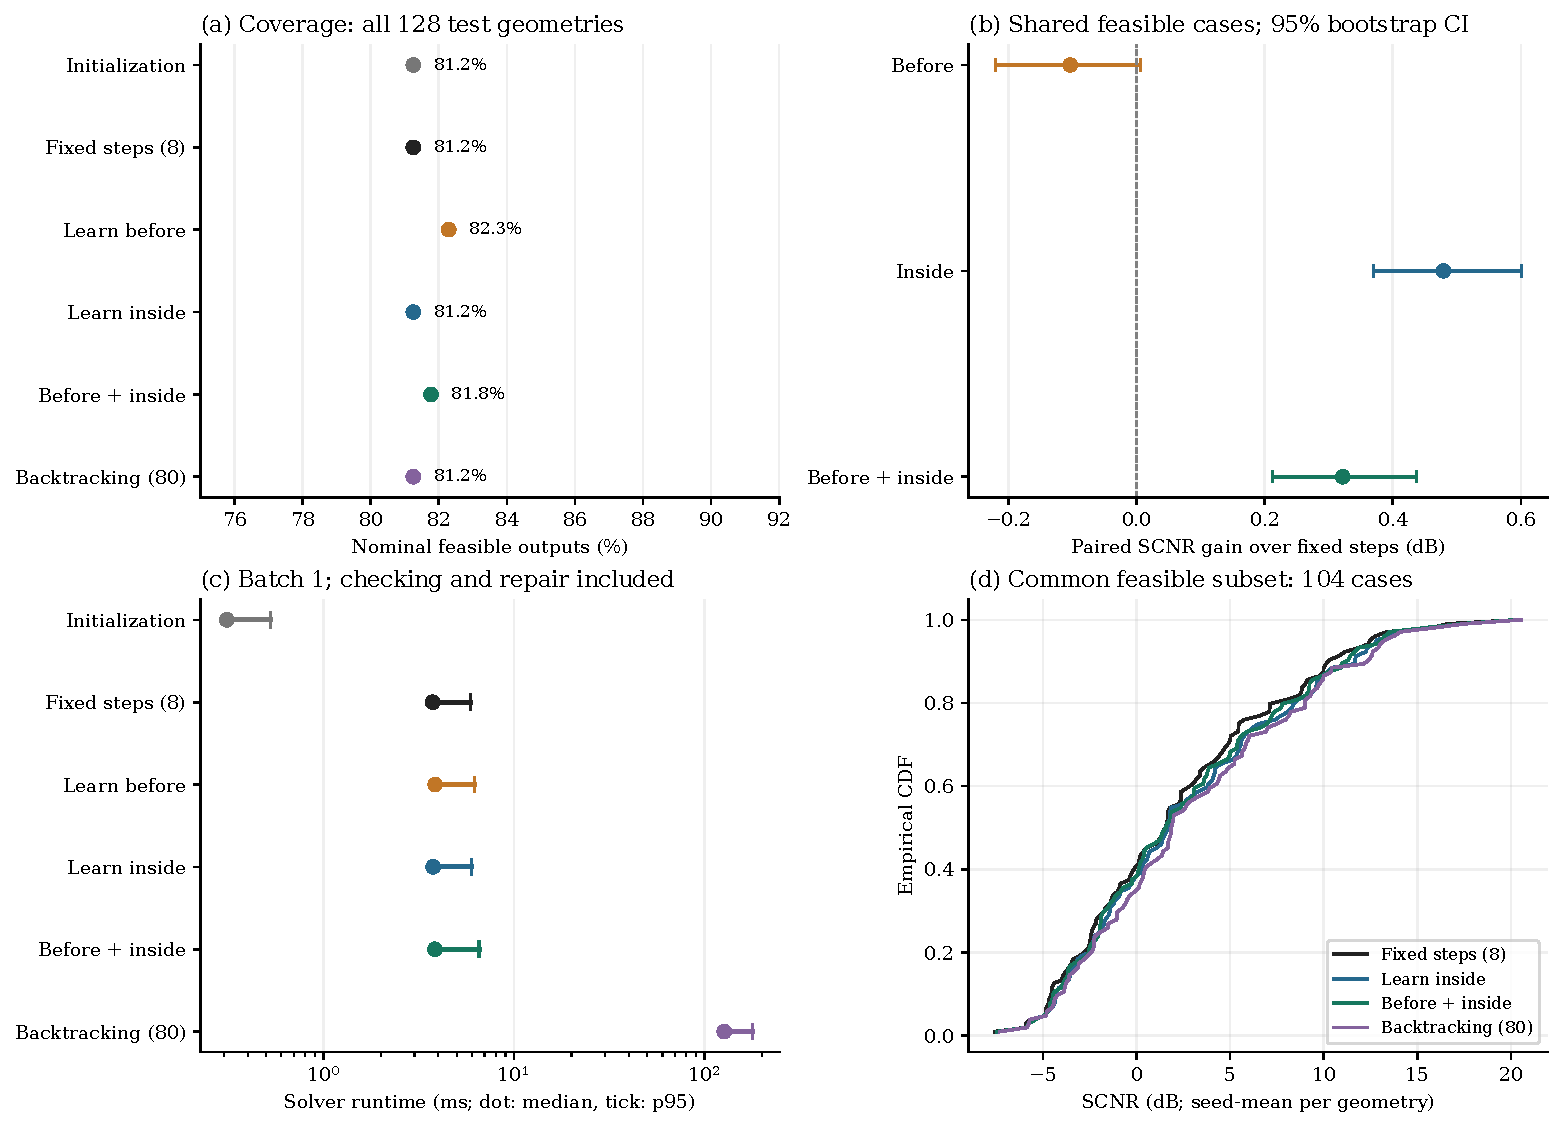
\includegraphics[width=\linewidth]{results/simulation-summary.pdf}
\caption{Measured results from this prototype. Coverage retains failed cases; paired gains and the CDF use shared-feasible subsets. Confidence intervals resample geometries with trained models held fixed.}\end{figure}

\subsection{Clutter shift and dimension diagnostic}
The shifted test multiplies clutter RCS by three and concentrates clutter around the target; it also uses new user and target geometries. It is therefore not a paired intervention on the same scenes. Inside-only learning retained an average paired improvement of 0.465 dB over fixed steps on their shared feasible cases; combined learning gave 0.323 dB. Neither result establishes robust feasibility under unknown channel or clutter errors.
An additional frozen-seed-17 diagnostic changes $(N,M)$ from $(6,12)$ to $(12,24)$ and $(24,48)$, retaining $K=2$ and fixed physical apertures. It uses 32 fresh instances at each size, with no retraining. It tests execution and limited dimension transfer only; it does not validate arbitrary-user scalability or array hardware physics.
\begin{center}\small\begin{tabular}{rrlrr}\toprule
$N$ & $M$ & Method & Feasible / 32 & Median (ms)\\\midrule
6 & 12 & fixed8 & 26 & 3.70 \\
6 & 12 & combined17 & 26 & 3.66 \\
12 & 24 & fixed8 & 32 & 4.07 \\
12 & 24 & combined17 & 32 & 4.09 \\
24 & 48 & fixed8 & 32 & 6.15 \\
24 & 48 & combined17 & 32 & 5.98 \\
\bottomrule\end{tabular}\end{center}
An independent covariance check with 100,000 random symbol/scatterer draws produced SCNR relative error 0.0051 against the analytical expression. This checks the assumed ensemble covariance model, not its validity for measured clutter.
\begin{figure}[!htbp]\centering
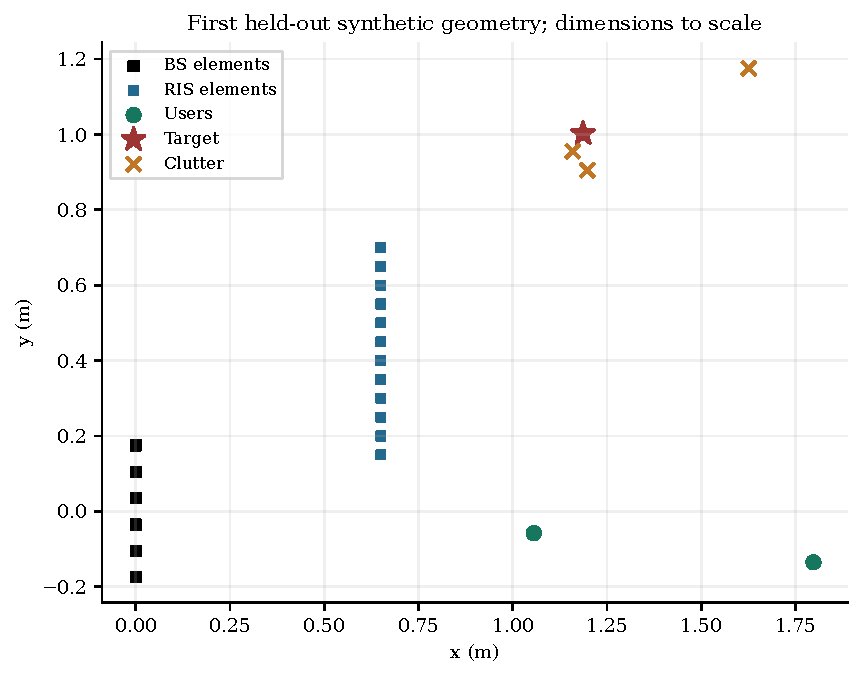
\includegraphics[width=.75\linewidth]{results/simulated-geometry.pdf}
\caption{Coordinates of the first held-out case used by the simulator. This figure is generated from the saved test dataset, not an illustrative performance claim.}\end{figure}


\section{What is established and what remains open}
The tests establish consistency of the analytical derivatives, receive-filter update, nominal fixed-direction power repair, and implemented comparisons for the specified synthetic model. Failed initialization is not a proof that no joint feasible solution exists. Conditional SCNR averages concern different accepted subsets unless a shared-feasible comparison is explicitly used.

The experiments do not establish uncertainty robustness, target detection probability, calibrated sensing accuracy, mobility performance, tail reliability of an operational service, hard real-time guarantees, or global optimality. The shifted-clutter test is a distribution-shift diagnostic, not a worst-case uncertainty certificate. A depth reduction relative to an 80-step reference does not prove superiority at equal wall-clock budgets.

The next implementation should first independently audit this model, introduce a stronger constrained reference solver, and add matched-time comparisons. A PyTorch implementation can then use implicit differentiation or controlled differentiation through linear solves, while verifying all real/complex gradient conventions against this NumPy reference. Expensive-block approximation should follow measured profiling, with residual checks and exact fallback. Finally, replace ideal information with estimated channels/clutter and a calibrated uncertainty model; only then investigate robust constraints, detection/tracking, and operational latency.

\bibliographystyle{ieeetr}\bibliography{reference}
\end{document}
